\documentclass[12pt,a4paper]{jarticle}
\usepackage[dvipdfmx]{graphicx}
\graphicspath{{../png/}}

\begin{document}
\section{水温変化のコンター}
\begin{figure}[hbtp]
    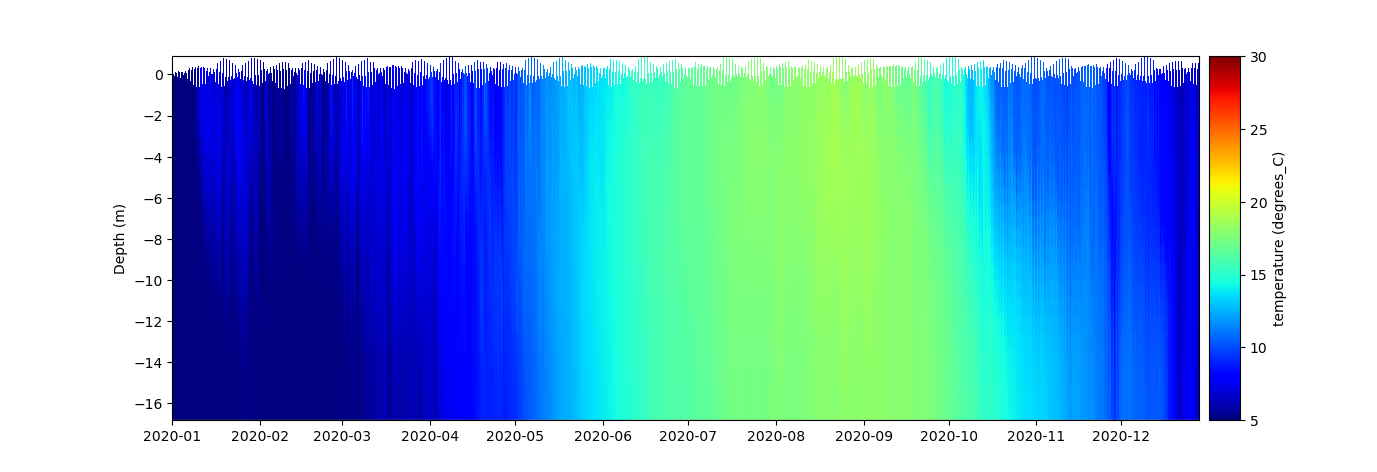
\includegraphics[keepaspectratio,width=180mm]{contour/Tokyo3_chiba1buoy.png}
    \caption{熱量2倍}
\end{figure}

\begin{figure}[hbtp]
    \centering
        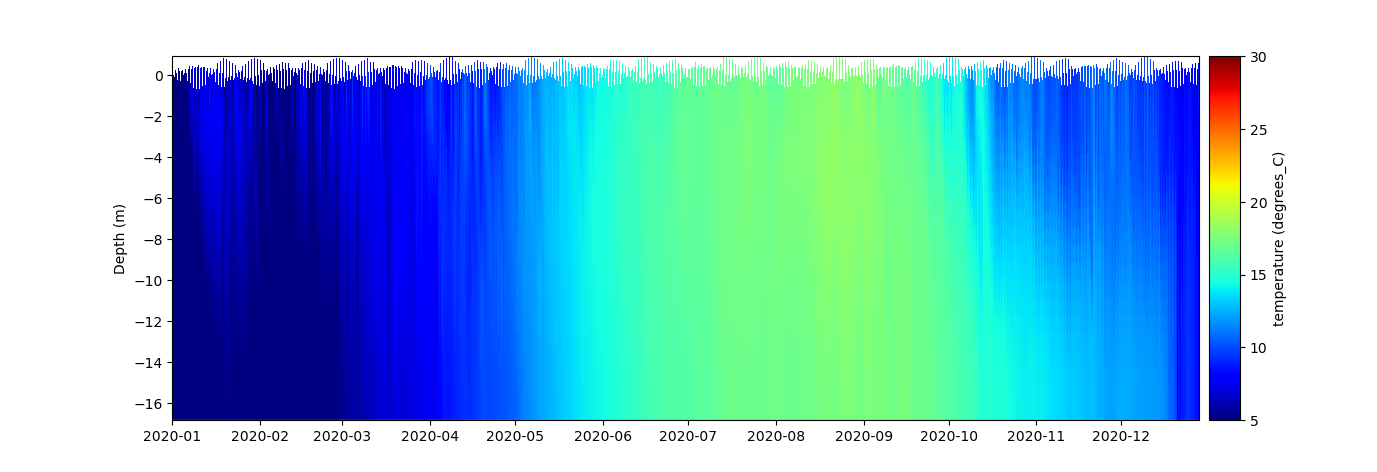
\includegraphics[keepaspectratio,scale=0.5]{contour/Tokyo4_chiba1buoy.png}
    \caption{熱量1倍}
\end{figure}

\begin{figure}[hbtp]
    \centering
        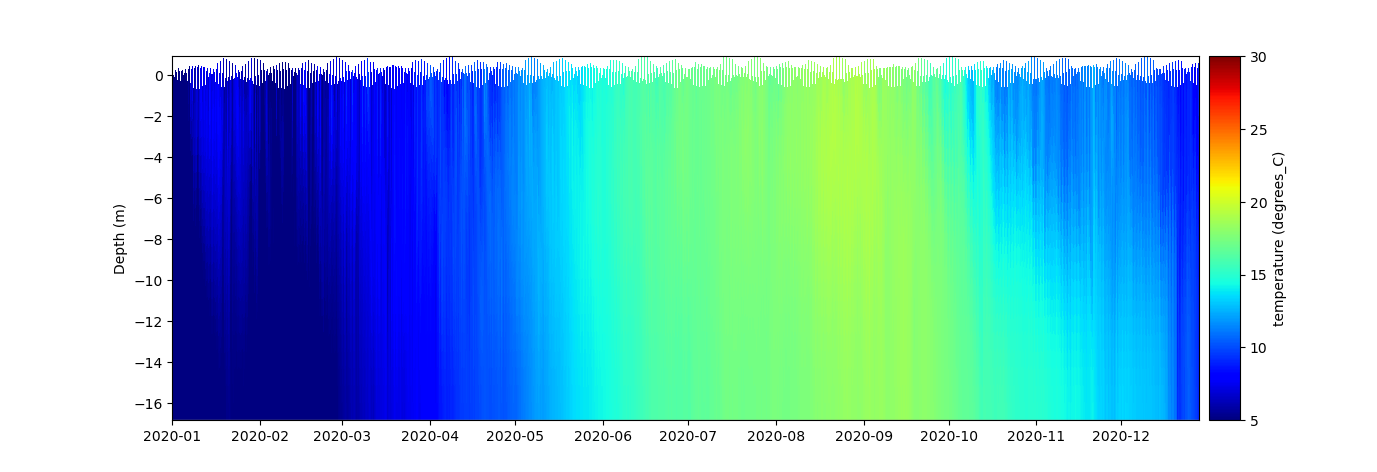
\includegraphics[keepaspectratio,scale=0.5]{contour/Tokyo5_chiba1buoy.png}
    \caption{熱量1.2倍}
\end{figure}

\newpage
\section{sigma layerごとでの水温変化}
\begin{figure}[hbtp]
    \centering
        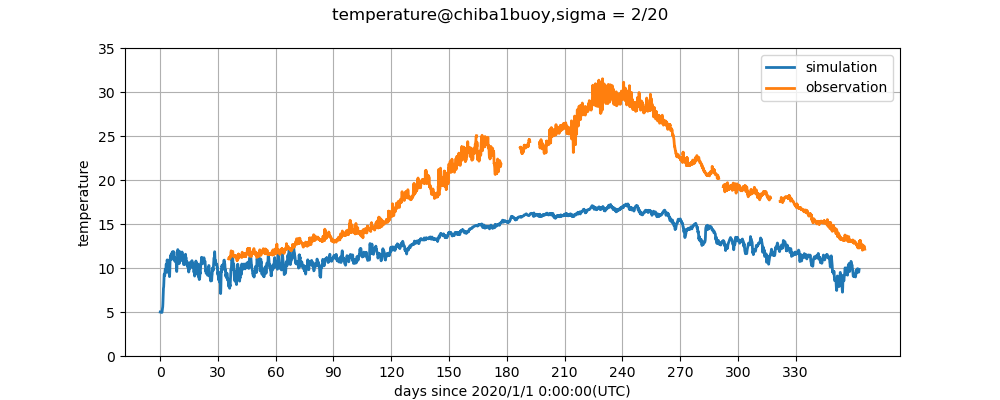
\includegraphics[keepaspectratio,scale=0.5]{Tokyo4/temperature_chiba1buoy_2_Tokyo4.png}
    \caption{siglay=2}
\end{figure}

\begin{figure}[hbtp]
    \centering
        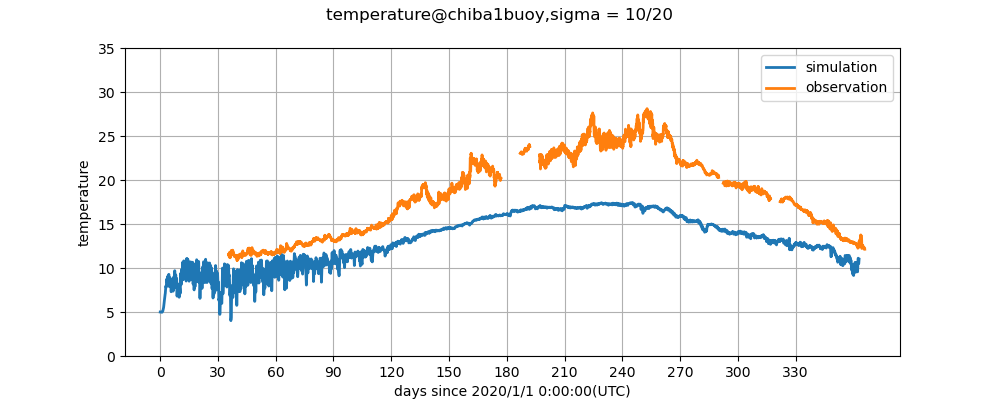
\includegraphics[keepaspectratio,scale=0.5]{Tokyo4/temperature_chiba1buoy_10_Tokyo4.png}
    \caption{siglay=10}
\end{figure}

\begin{figure}[hbtp]
    \centering
        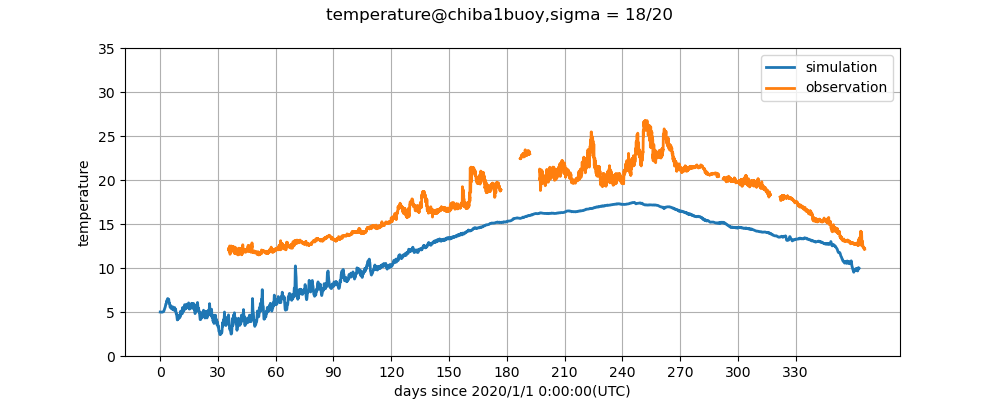
\includegraphics[keepaspectratio,scale=0.5]{Tokyo4/temperature_chiba1buoy_18_Tokyo4.png}
    \caption{siglay=18}
\end{figure}

        
\end{document}

